\chapter{Motion-Aware Unitを用いた1波長を入力とした紫外線像の全球時系列予測}
  \section{実験概要}
  この実験では入力、出力ともに211Åフィルターで得られたデータを利用した。
  これは 211Åフィルターで撮影された紫外線像が、コロナホールと活動領域といった、二つの太陽円盤上の大規模構造をバランスよく明瞭に表現し、本研究のモデルの効果検証に適していると考えたためである。
  モデルにはMotion-Aware Unitを用い、1波長のデータを入力として、全球の時系列予測を行った。
  この実験の概要を図\ref{fig:exp1_overview}に示す。

  \begin{figure}[htbp]
    \centering
    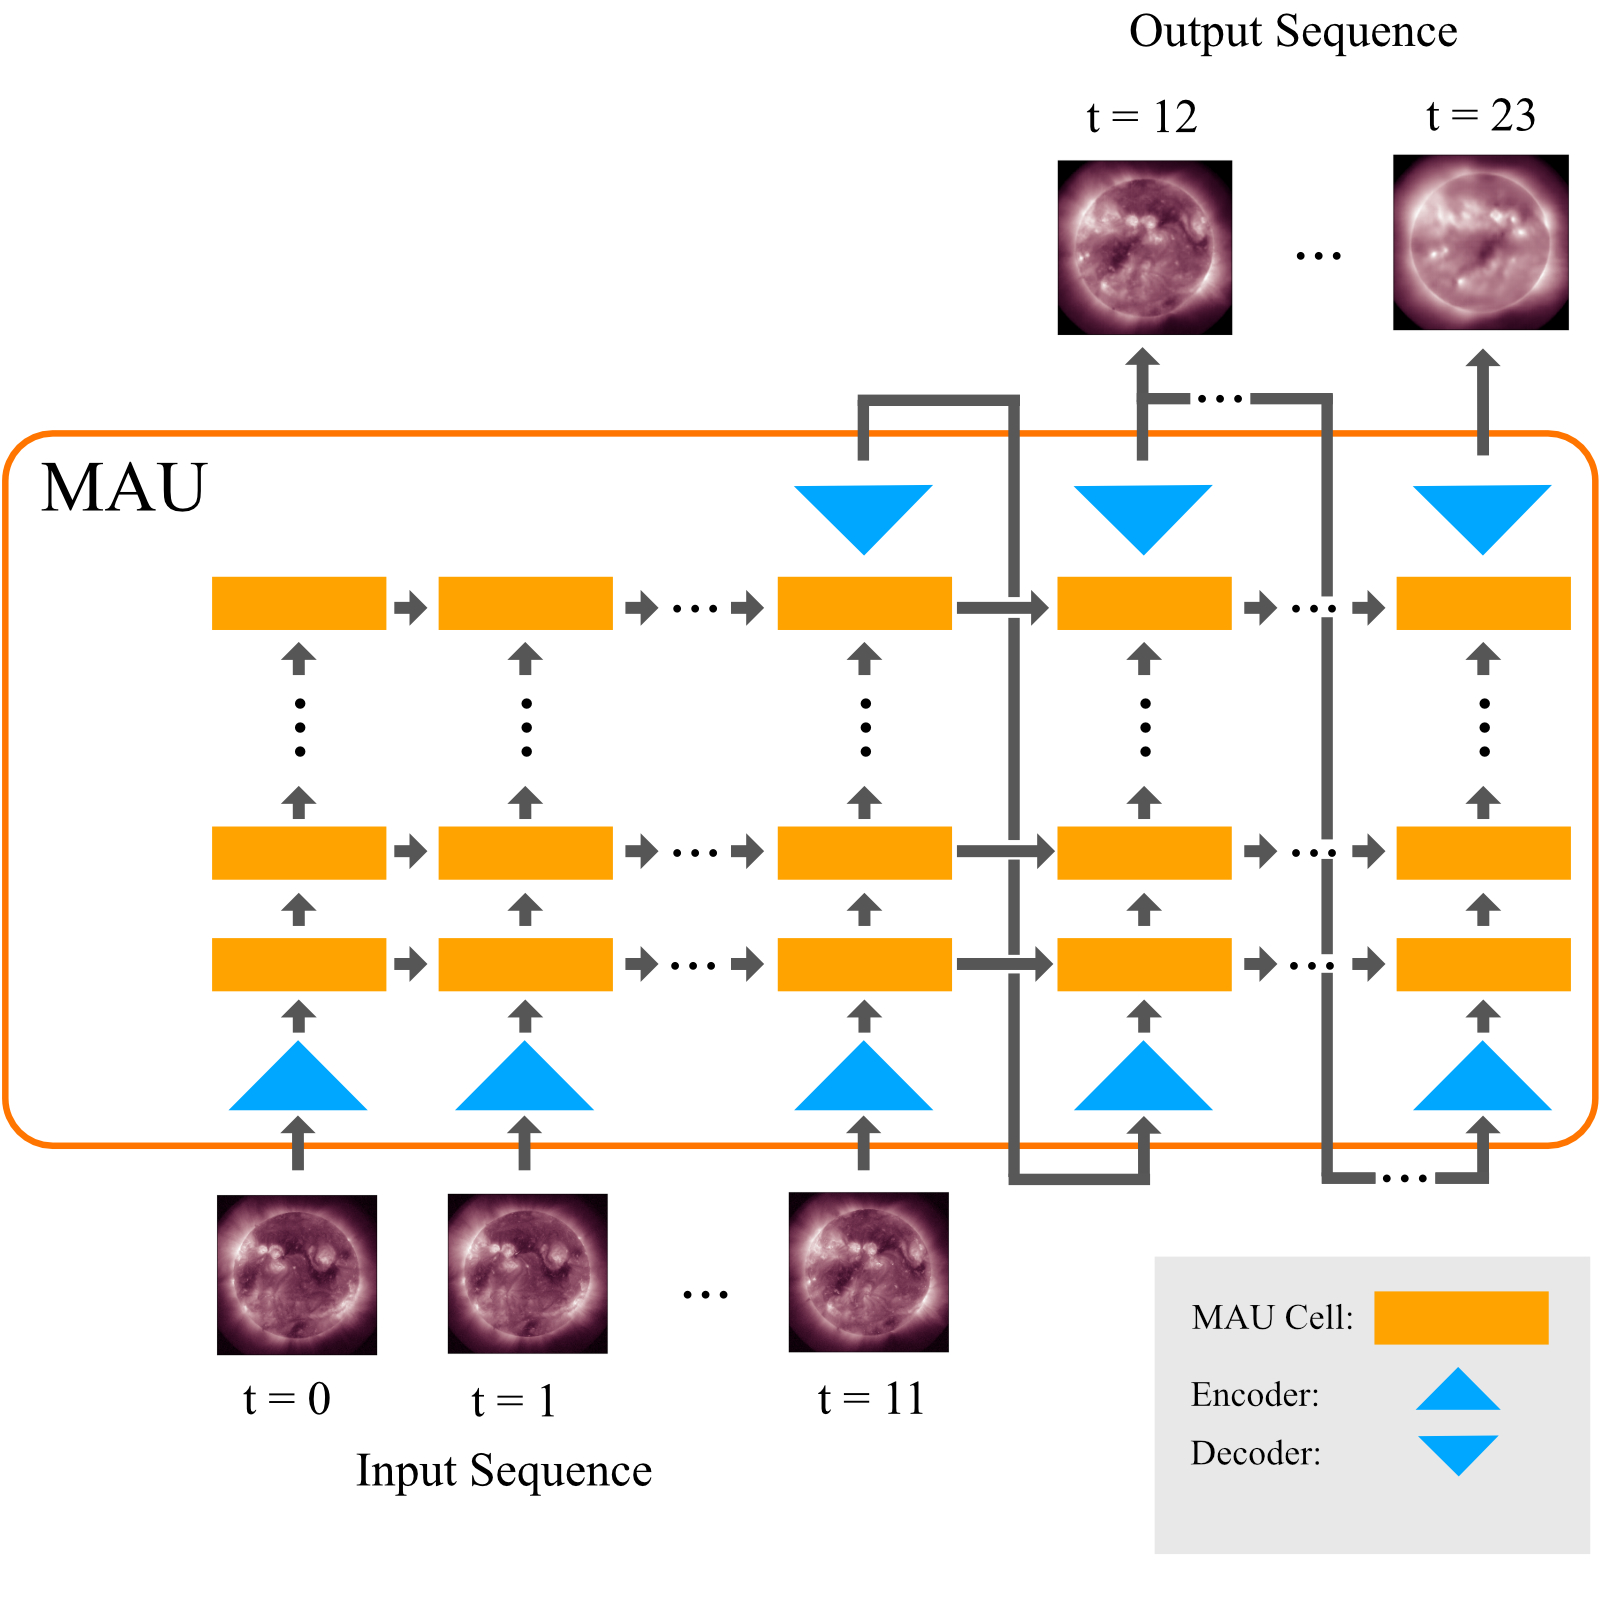
\includegraphics[width=\textwidth]{figures/exp1/exp1_concept.jpg}
    \caption{実験の概念図。モデルにはMotion-Aware Unitを用い、1波長のデータを入力として、全球の時系列予測を行った。}
    \label{fig:exp1_overview}
  \end{figure}

  \section{実験設定}
    各ハイパーパラメータの設定を表\ref{tab:exp1_hyperparameters}に示す。
    バッチサイズは実験的に決定し、最も安定的に最終的に良好な精度を達成できた値を採用した。
    また、エポック数は100とした。学習率は0.0005とした。MAU Cell数は、Chang et al. (2019) \cite{chang2021mau} の実験設定を参考に、16とした。
    学習時間の短縮およびメモリ使用量の削減のため、学習時にはAutomatic Mixed Precision (AMP)\ref{micikevicius2017mixed}を用いた。
    これは、単精度浮動小数点演算と半精度浮動小数点演算を適切に混在させることで、モデル性能をほとんど落とさずに計算資源を節約し学習を高速化する手法である。
    GPUはNVIDIA RTX A6000を用いた。
    \begin{table}[htbp]
      \centering
      \begin{tabular}{lc}
      \hline
      ハイパーパラメータ & 値 \\
      \hline\hline
      バッチサイズ & 4 \\
      \hline
      エポック数 & 100 \\
      \hline
      学習率 & 0.0005 \\
      \hline
      損失関数 & MSE \\
      \hline
      チャンネル & 1 \\
      \hline
      カーネルサイズ & (5, 5) \\
      \hline
      MAU Cell数 & 16 \\
      \hline
      \end{tabular}
      \caption{本実験でのハイパーパラメータ設定}
      \label{tab:exp1_hyperparameters}
    \end{table}

  \section{学習の推移}
  学習は図\ref{fig:exp1_learn_progress}のように推移した。
  学習損失は全体的に安定して推移し、検証損失は時折急激に値が増加しているが、全体的には減少している。
  学習の完了までには約12時間を要した。
  \begin{figure}[htbp]
    \centering
    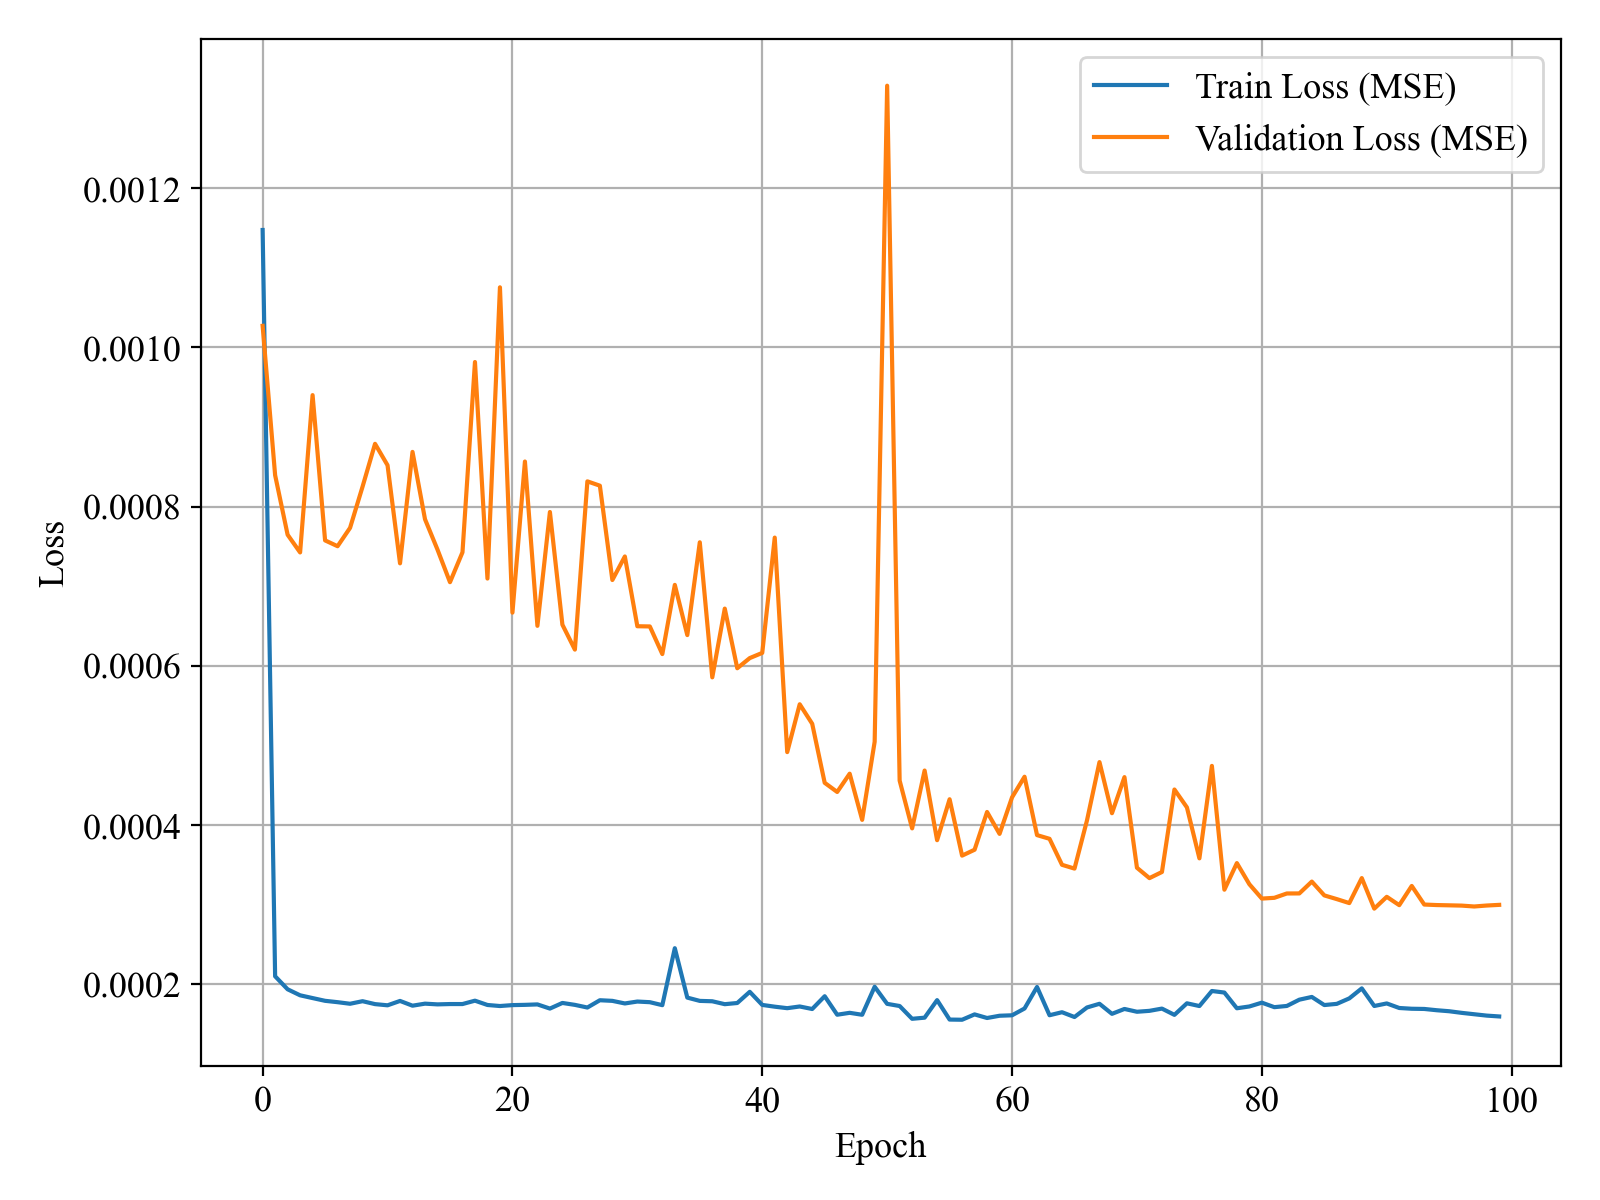
\includegraphics[width=0.9\textwidth]{figures/exp1/loss.png}
    \caption{本実験での、学習データ、検証データでの損失関数の推移。学習の損失は安定している。検証の損失は振動しながら減少している。}
    \label{fig:exp1_learn_progress}
  \end{figure}

  \section{実験結果}
    図\ref{fig:exp1_gt}および図\ref{fig:exp1_pd}に、この実験での出力例を示す。
    これは学習データに含まれない期間のテストデータである。
    \begin{figure}[htbp]
      \centering
      %\vspace*{-4cm} % 上の余白を調整
      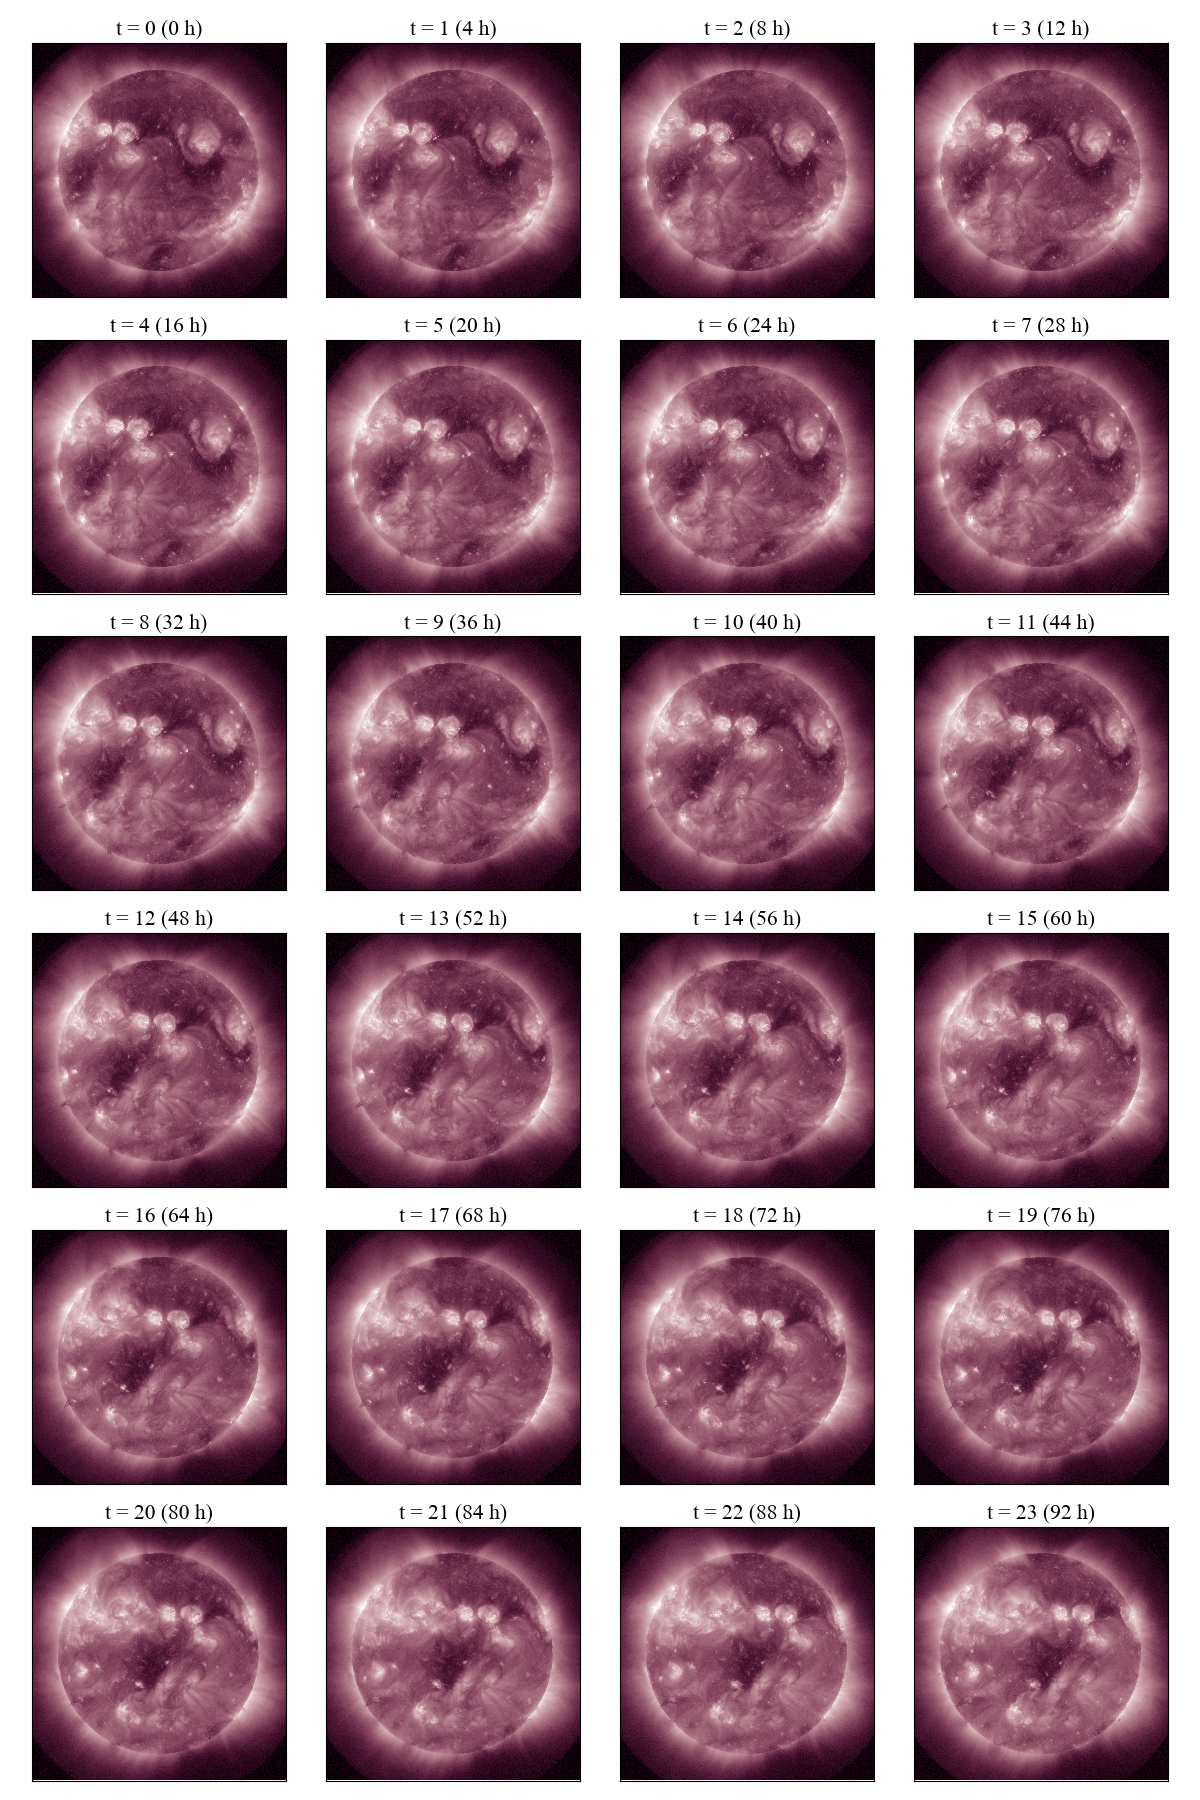
\includegraphics[width=0.95\textwidth]{figures/exp1/gt.png}
      \caption{実際の観測画像の例。2022年10月28日0時から2022年11月1日20時までの期間から4時間毎にサンプリングされている。このt=0からt=11までをモデルに入力データとして渡している。モデルはその入力データを元に、t=12からt=23の12枚の画像を予測する。t=12以降の実際の観測画像はモデルに渡されない。}
      %\vspace{-1cm} % 下の余白を調整
      \label{fig:exp1_gt}
    \end{figure}
    \begin{figure}[htbp]
      \centering
      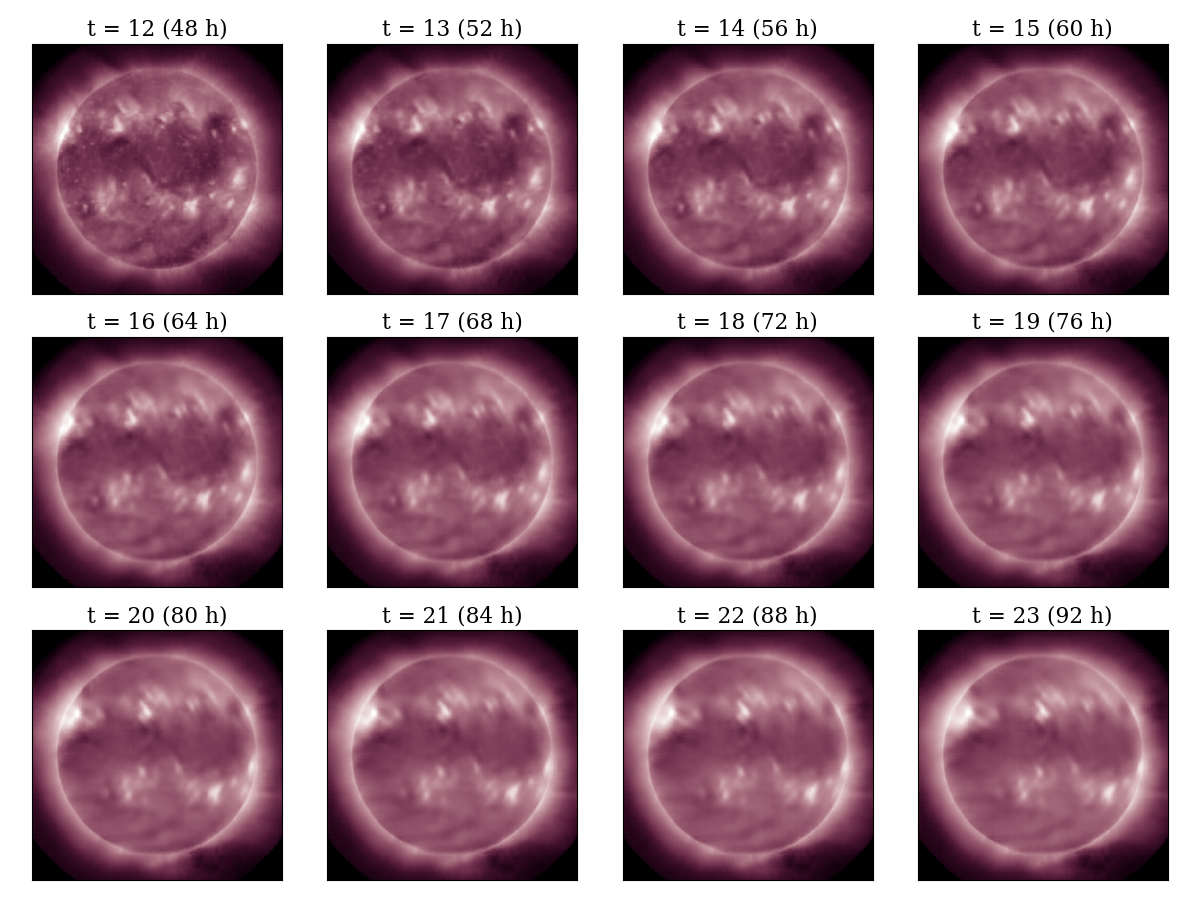
\includegraphics[width=0.95\textwidth]{figures/exp1/pd.png}
      \caption{MAUによる予測画像。対応するタイムステップtの観測画像(図\ref{fig:exp1_gt})と比較することでモデルの再現度を視覚的に評価することができる。大規模な構造は概ね実際の観測画像と合致している。モデルの特性により、時間経過とともに少しずつ予測が不安定になり、ぼやけた見た目になる。}
      \label{fig:exp1_pd}
    \end{figure}
    モデルの出力は、視覚的には実際の観測画像と概ね合致しており、特に自転による大規模構造の移動といった顕著な時間的特徴は再現できていることがわかる。

    動画予測の精度を評価するために、太陽の輝度強度の再現性を定量的、またまたは視覚的に評価する。
    これは、Nishizuka et al. (2018) \cite{nishizuka2018deep} や〜〜〜などの、太陽画像から太陽イベントを予測する先行研究では、その画像中の輝度強度を主要な特徴量として採用していることに基づく。
    この輝度強度の再現性の評価を、さまざまな条件下で行った。はじめに全球での評価を行い、次に経度依存性の評価を行った。最後に、東側リムから出現する活動領域に対する視覚的評価を行った。

% *************************************************************************************************************

    \subsection{全球での評価}
      はじめに全球での評価を行った。
      この評価では、まず輝度強度の平均値と実際の平均値との誤差、構造的類似度(Structual Similarity, SSIM)を計算した。さらに単純差動回転モデルとの比較も行った。
      これらの値の時間経過に対する変化を観察し、より不確定性の高い将来の予測に対しても動画予測モデルが有効であるかを検証した。
      
      \subsubsection{平均輝度の再現}
        \paragraph{平均輝度の絶対誤差の計算}
          テストセット全体における、ある時間ステップtの平均輝度の絶対誤差を以下のように計算した。
          \begin{align}
            \bar{E}_{t} & = \frac{1}{N} \sum_{i=1}^{50} | \bar{I}_{\text{Prediction}_{i,t}} - \bar{I}_{\text{Actual}_{i,t}} |
          \end{align}
          ここで、iはテストセットのインデックスを表す。また、\( \bar{I}_{\text{Prediction}_{i,t}} \)は、テストセットi、時間ステップtにおける、モデルから生成された画像から計算された平均輝度を表し、\( \bar{I}_{\text{Actual}_{i,t}} \)は、実際の画像から計算された平均輝度を表す。
          平均輝度は全球(画像中の太陽の球面)に対してのみ行い、画像中の背景や外縁部からはみ出すコロナなどはその計算に含まれない。
          背景から全球に対して切り出される部分は、図\ref{fig:exp1_fulldisk_crop}に示されている。
          この全球の定義および計算は、取得したFITSファイルのヘッダーに記載される太陽の中心および半径に基づいている。
          \begin{figure}[htbp]
            \centering
            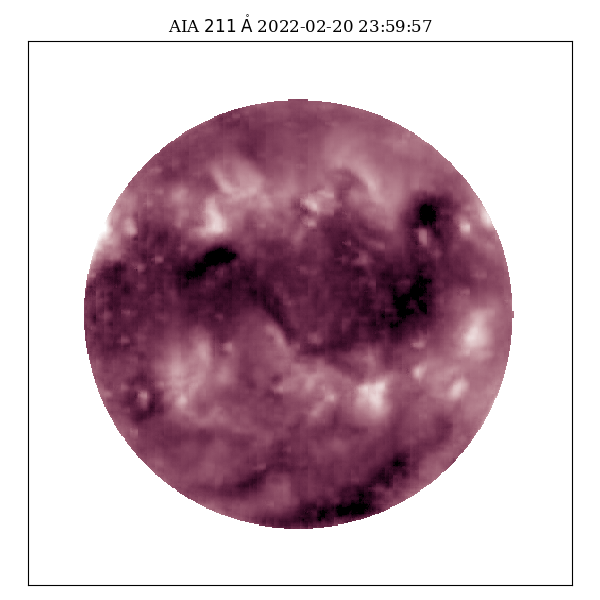
\includegraphics[width=0.6\textwidth]{figures/exp1/crop_map.png}
            \caption{生成した画像から全球部分のみ切り出した画像の例。この部分にのみ平均輝度を計算する。}
            \label{fig:exp1_fulldisk_crop}
          \end{figure}

          モデルの出力の全球での平均輝度と、実際の観測画像との誤差の推移を図\ref{fig:exp1_mean_intensity_line}に示す。
          これは、50のテストセットに対して、各テストセットに含まれる各画像の全球での平均輝度を計算し、その時間ステップごとの平均値を取ったものである。
          輝度の推移のみから特定の傾向を見出すことは難しいが、全体として平均絶対誤差は4\%以下に収まっている。
          \begin{figure}[htbp]
            \centering
            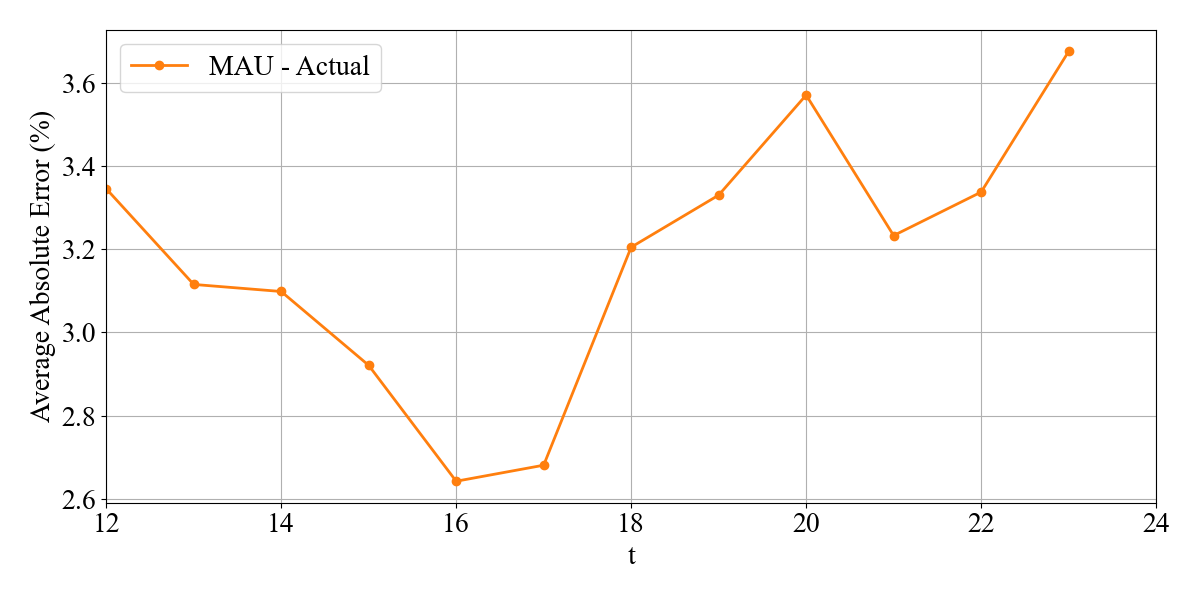
\includegraphics[width=\textwidth]{figures/exp1/error.png}
            \caption{MAUによるテストセットの予測画像と実際の観測画像の平均絶対誤差の時間推移。横軸が時間ステップ、縦軸が平均絶対誤差を表す。時間ステップを経る毎に誤差は単調に上昇していくが、その誤差は最終タイムステップでも5\%以下にとどまっている。}
            \label{fig:exp1_mean_intensity_line}
          \end{figure}
          
          さらに、入力シークエンスの最後から48時間後の画像の全球での平均輝度と、実際の観測画像との差異を観察する。その散布図\ref{fig:exp1_mean_intensity_scatter}に示す。
          このタイムステップは、出力の最後のタイムステップであり、最も不確定性の高い予測である。
          相関係数は0.97であり、非常に良好な値である。実際の観測画像の平均輝度の高低に関わらず、高い精度で平均輝度を再現できていることがわかる。
          \begin{figure}[htbp]
            \centering
            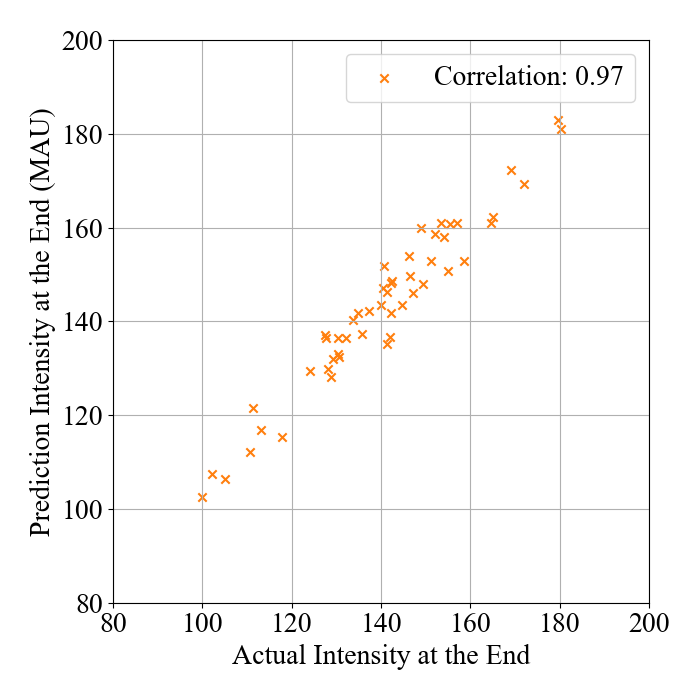
\includegraphics[width=0.6\textwidth]{figures/exp1/intensity_scatter_gt_pd.png}
            \caption{テストセットの最終ステップにおける全球平均輝度の予測対実測の散布図。縦軸がMAUによる予測から計算された平均輝度強度、横軸が実際の観測画像から計算された平均輝度強度を表す。計算された相関係数は0.97である。}
            \label{fig:exp1_mean_intensity_scatter}
          \end{figure}

        \paragraph{単純差動回転モデルとの比較}
          モデルの予測性能をさらに詳細に評価するために、シンプルな差動回転モデルとの比較を行った。
          目視や、平均輝度から、モデルの出力は実際の観測画像と概ね合致しており、特に自転による構造的変化などの主要な時間的特徴を再現できていることがわかった。
          ここでは、単純差動回転シミュレーションモデルによる出力と、我々のモデルの出力の再現精度の比較を行う。
          これにより、モデルが単に自転を予測しているのではなく、より複雑な時間的変化を予測できているかを検証した。

          太陽は自転するが、その実体は流体であるため、緯度によって自転速度が異なる。極付近の自転周期は約35日であるが、赤道付近では約25日である。この現象を差動回転と呼ぶ。
          差動回転をシミュレーションする研究は盛んに行われているが、ここでは回転速度を緯度依存としてモデル化するHoward et al. (1990) \cite{howard1990solar}の差動回転モデルを用いた。
          このモデルは、Heliographic緯度\(\theta\)に対する回転速度\(\omega(\theta)\)を以下のように定義する:
          
          \begin{align}
            \omega(\theta) &= A + B \sin^{2}(\theta) + C \sin^{4}(\theta) \\
            \text{where} \quad A &= 2.894 \, \mu\text{rad/s}, \\
            B &= -0.428 \, \mu\text{rad/s}, \\
            C &= -0.370 \, \mu\text{rad/s}
          \end{align}
          このモデルはSunpyに実装されており、\textit{physics.differential\_rotation}というモジュールとして提供されている。
          このモジュールによる画像の生成は、全球の各ピクセルに対して、そのピクセルの緯度に対する回転速度を計算し、その速度で西に向かって各ピクセルを移動させることで行われる。
          この単純差動回転モデルによるシミュレーションの例を図\ref{fig:exp1_sdr_example}に示す。
          比較は、単純差動回転モデルによるシミュレーションと、実際の観測画像との平均輝度の絶対誤差を計算し、それを前述の動画予測によるものと比較することで行った。
          この誤差の推移を図\ref{fig:exp1_sdr_line}に示す。単純差動回転モデルは時間経過とともに誤差が単調に増加するが、動画予測モデルは最終タイムステップにおいても誤差が4\%以下に収まっている。
          t=1 \~ 4の間は、単純差動回転モデルの方が誤差が小さいが、それ以降は逆転し、動画予測モデルの方が誤差が小さくなっている。
          このことから、動画予測モデルは、単純差動回転モデルよりも、より時間経過に対して堅牢であることがわかる。
          \begin{figure}[htbp]
            \centering
            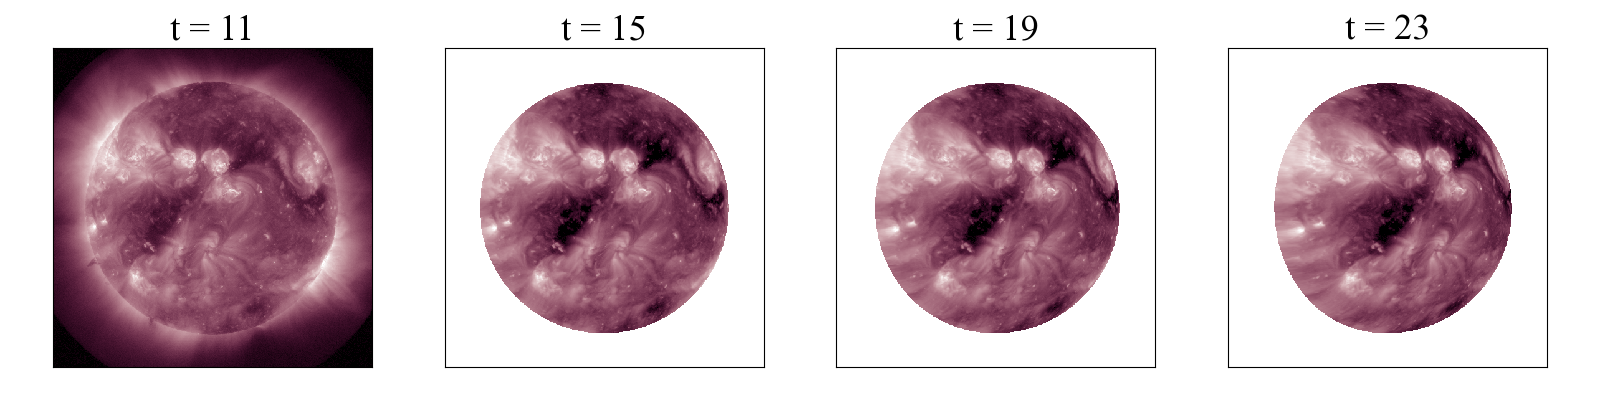
\includegraphics[width=1.1\textwidth]{figures/exp1/sdr.png}
            \caption{Howard (1990)による差動回転モデルによるシミュレーションの例。入力シークエンスの最終入力(t=11)(左)をもとに、各ピクセルに式(4.2)を適用し移動させることで画像を生成する。全球面以外の背景には計算されない。}
            \label{fig:exp1_sdr_example}
          \end{figure}

          \begin{figure}[htbp]
            \centering
            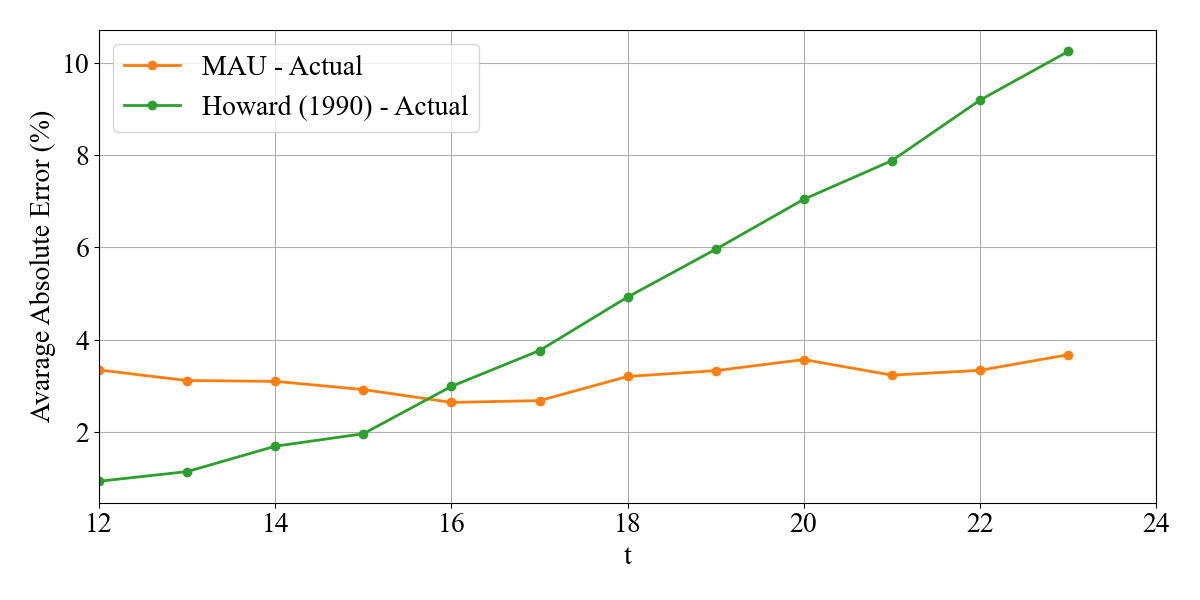
\includegraphics[width=\textwidth]{figures/exp1/error_dr.png}
            \caption{MAUによるテストセットの予測画像と実際の観測画像の平均絶対誤差(オレンジ)と、単純差動回転モデルと実際の観測画像の平均絶対誤差(緑)。}
            \label{fig:exp1_sdr_line}
          \end{figure}
          
          さらに、出力シークエンスの最後のタイムステップにおいて、単純差動回転モデルによるシミュレーションと、実際の観測画像との差異を観察し、動画予測モデルによる出力と比較した。
          その散布図\ref{fig:exp1_sdr_scatter}に示す。
          単純差動回転モデルによるシミュレーションの平均輝度と、実際の観測画像の平均輝度は、相関係数では0.85である。
          データ点が全体的に左上に偏っていることから、単純差動回転モデルは、実際の観測画像よりも平均輝度を高く予測していることがわかる。
          一方で、前述のように、動画予測モデルによる出力の平均輝度と、実際の観測画像の平均輝度は、相関係数では0.97である。
          こことから、やはり最終タイムステップでの予測においても、動画予測モデルは単純差動回転モデルよりも高い精度で平均輝度を再現できていることがわかる。
          \begin{figure}[htbp]
            \begin{subfigure}[b]{0.55\textwidth}
              \centering
              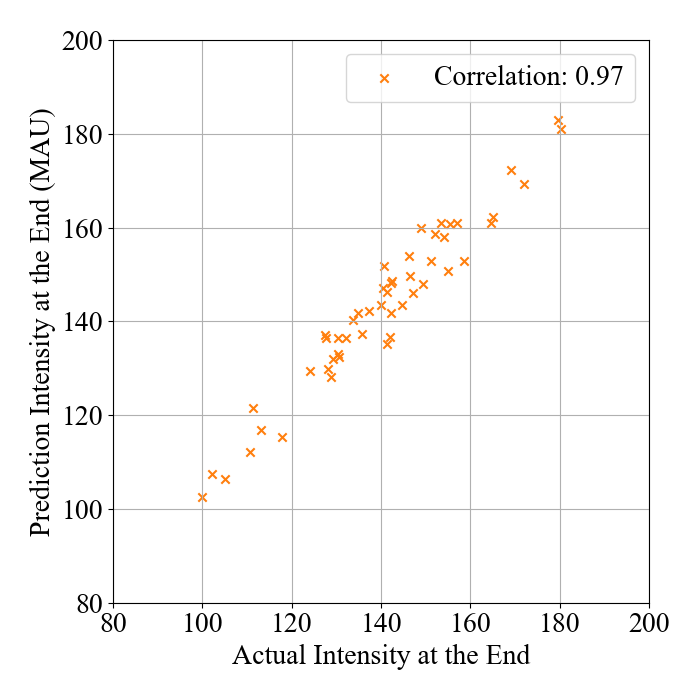
\includegraphics[width=\textwidth]{figures/exp1/intensity_scatter_gt_pd.png}
              \caption{MAUによる、テストセットの最終ステップにおける全球平均輝度の予測対実測の散布図。計算された相関係数は0.97である。}
            \end{subfigure}
            \begin{subfigure}[b]{0.55\textwidth}
              \centering
              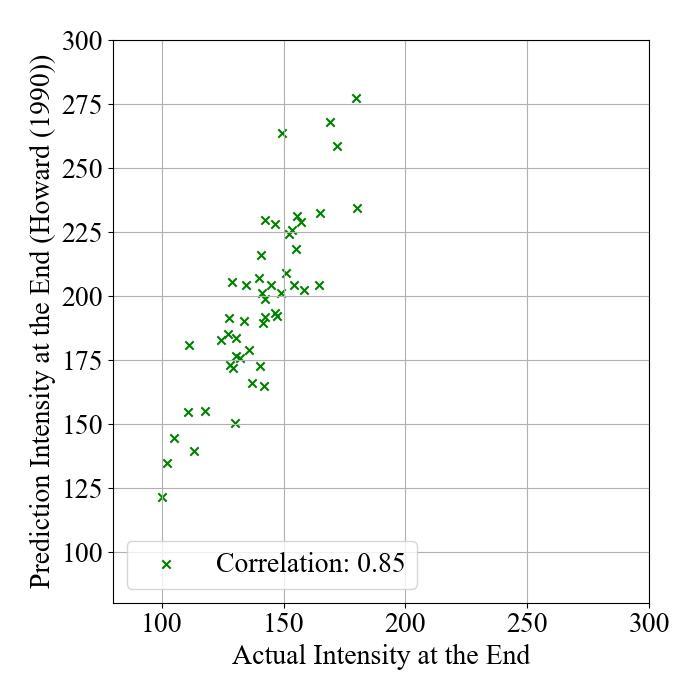
\includegraphics[width=\textwidth]{figures/exp1/intensity_scatter_gt_dr.png}
              \caption{単純差動回転モデルによる、テストセットの最終ステップにおける全球平均輝度の予測対実測の散布図。計算された相関係数は0.85である。}
            \end{subfigure}
            \label{fig:exp1_sdr_scatter}
            \caption{予測対実測の散布図。縦軸が予測から計算された平均輝度強度、横軸が実際の観測画像から計算された平均輝度強度を表す。}
          \end{figure}

      \subsubsection{画像類似度}
        画像内での構造的再現度とその時間的変化を評価するために、モデルの出力と対応する時間ステップの実際の観測画像の間のSSIMを計算した。
        SSIMは、画像の品質評価を目的として、Wang et al. (2004)\cite{wang2004image}で提案された。
        SSIMは特に構造情報が重要とされる医療画像や衛星画像のような分野で広く使用されている。従来の平均二乗誤差(MSE)やピーク信号対雑音比(PSNR)と比較して、SSIMは人間の視覚システムにより近い知覚品質を提供する。
        従来の手法とは異なり、SSIMは画像の輝度、コントラスト、構造の三つの比較を基にしている。
        SSIMの定義は以下の通りである:
        \begin{equation}
          SSIM(x, y) = \frac{(2\mu_x \mu_y + C_1)(2\sigma_{xy} + C_2)}{(\mu_x^2 + \mu_y^2 + C_1)(\sigma_x^2 + \sigma_y^2 + C_2)},     
        \end{equation}
        ここで、$x$と$y$は比較される二つの画像、$\mu_x$、$\mu_y$はそれぞれの画像の平均輝度、$\sigma_x^2$、$\sigma_y^2$はそれぞれの分散、$\sigma_{xy}$は共分散である。$C_1$と$C_2$は安定性のための小さな定数である。
        
        テストセット全体における、ある時間ステップtのSSIMの平均を以下のように計算した。
        \begin{align}
          \bar{SSIM}_{t} & = \frac{1}{N} \sum_{i=1}^{50} \text{SSIM}_{i,t}
        \end{align}

        画像類似度も、全球での平均輝度と同様に、全球に対してのみ行い、画像中の背景や外縁部からはみ出すコロナなどはその計算に含まれない。
        また、平均輝度の場合と同様に、単純差動回転モデルとの比較も同時に行った。
        このように計算されたSSIMの時間推移を図\ref{fig:exp1_ssim_line}に示す。
        MAUのSSIM、単純差動回転モデルによるSSIMは、共に時間経過とともに単調に減少していくが、MAUによるSSIMの方が、最終タイムステップにおいても0.94を超えているのに対し、単純差動回転モデルによるSSIMは0.92程度である。
        また、t=12\~16の初期段階では、単純差動回転モデルの方がSSIMが高いが、それ以降は逆転し、MAUによるSSIMの方が高い。
        この傾向は平均輝度の場合と概ね同様であり、やはりMAUによる予測は画像類似度においてもその低下が緩やかである。 
        
        \begin{figure}[htbp]
          \centering
          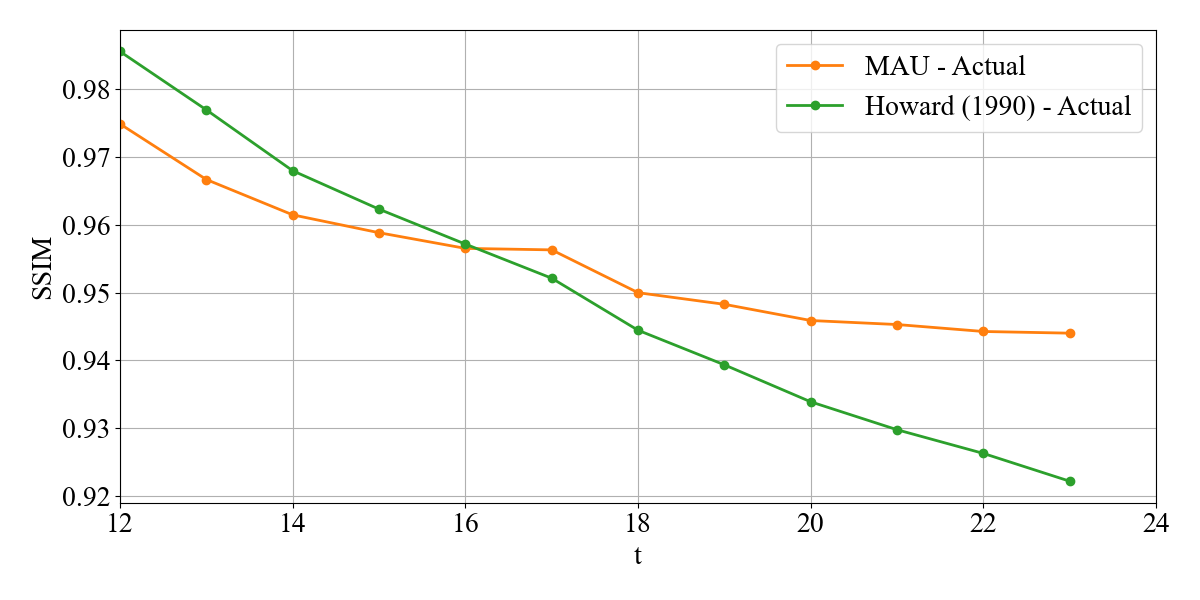
\includegraphics[width=\textwidth]{figures/exp1/average_ssim.png}
          \caption{テストセットでのSSIMの時間推移。SSIMは0から1の値を取り、二つの画像が類似するほど1に近づく。横軸が時間ステップ、縦軸がSSIMを表す。}
          \label{fig:exp1_ssim_line}
        \end{figure}
      
% *************************************************************************************************************

    \subsection{経度依存性の評価}
        さらに、予測性能が経度ごとにばらつきがあるかを確認するために、経度ごと予測の再現度を評価した。
        具体的には、Heliographic Stonyhurst座標系における経度-90°から90°までの半球を、36°ごとに5つのセクターに分割した。
        分割の概念図を図\ref{fig:exp1_division_concept}に示す。
        評価指標には、全球の場合と同様に、平均輝度の平均絶対誤差と、SSIMによる画像類似度を用いた。また、それぞれの評価において、単純差動回転モデルとの比較も行った。
        
        \begin{figure}[htbp]
          \centering
          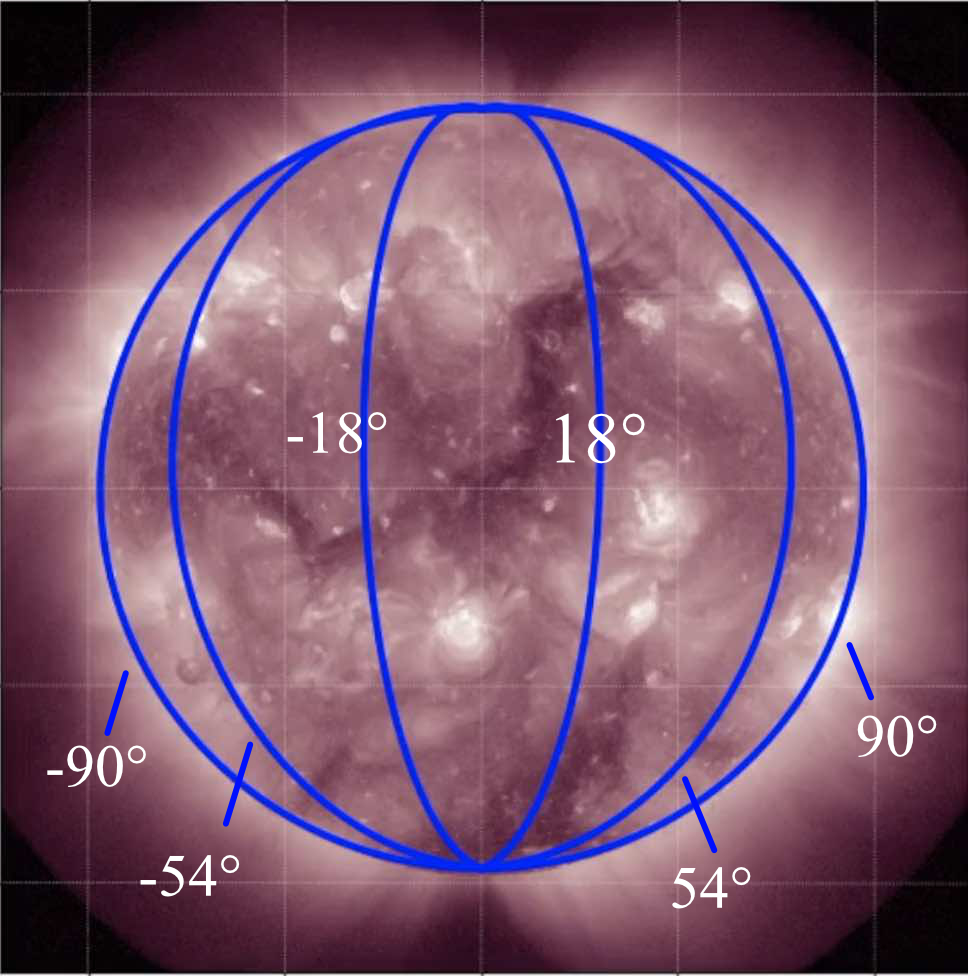
\includegraphics[width=0.65\textwidth]{figures/exp1/devision_caption.jpg}
          \caption{分割の様子を示した図。Heliographic Stonyhurst経度-90°から90°までの半球を、36°ごとに5つのセクターに分割した。}
          \label{fig:exp1_division_concept}
        \end{figure}

        \subsubsection{平均輝度の再現}
          ここでは、全てのテストセットで各セクターごとの平均輝度を計算し、対応する時間ステップの実際の観測画像との間の絶対誤差を計算した。
          ここで、ある時間ステップt、ある経度セクターlにおける平均輝度の絶対誤差\( \bar{E}_{l,t} \)は以下のように定義される:
          \begin{align}
            \bar{E}_{l, t} & = \frac{1}{N} \sum_{i=1}^{50} | \bar{I}_{\text{Prediction}_ {i, l, t}} - \bar{I}_{\text{Actual}_{i, l, t}} | \\
          \end{align}
          ここで、iはテストセットのインデックスを表す。また、\( \bar{I}_{\text{Prediction}_{i, l, t}} \)は、テストセットi、時間ステップt、経度セクターlにおける予測された平均輝度を表し、\( \bar{I}_{\text{Actual}_{i, l, t}} \)は、実際の平均輝度を表す。  
            
          このように計算された誤差率の時間推移を図\ref{fig:lng_error}に示す。
          単純差動回転モデルとの比較を行っている。
          
          \paragraph{経度-90度から-54度}
          -90度から-54度のセクターは、東の外縁部(画像に向かって左側)の領域である。
          太陽は東から西に向かって回転する。そのため、時間が経過するにつれて、東側の外縁部では、太陽の新しい表面が全球面に観測されるようになる。
          またこのセクターでは、観測者である望遠鏡に対して角度がきつく、実際の太陽表面の面積に対して観測できる面積が小さい。
          しかし、時間が経過し表面が太陽の中心経度に向かうにつれて、観測される面積は大きくなることから、この領域を正確に予測するには、少ない情報から詳細な予測を行う必要がある。
          このようなタスクはしばしば困難であり、シンプルなモデルで正確に予測することは難しいと考えられる。
          この領域に対する誤差の推移を図\ref{fig:lng_error_1}から検証すると、MAUによる予測は、最終タイムステップで20\%程度と、全球平均の誤差率と比べると高くなっている。
          一方で、単純差動回転モデルによる予測は、最終タイムステップで45\%程度であり、また全タイムステップにおいて、MAUによる予測よりも誤差率が高くなっている。
          このことから、不確実性が高い東側外縁部の領域に対しても、MAUは有効な予測能力を持っていることがわかる。この点については、後述する東側外縁部に対する視覚的評価でも確認する。

          \paragraph{経度-54度から-18度}
          -54度から-18度のセクターは、東側の中心部の領域である。
          この領域は、東側外縁部と比べると、観測される面積が大きいため、より予測は容易になるものの、時間経過によって東側外縁部から移動してくる表面を予測しなければならないため、一定の難しさがある。
          


          \begin{figure}[htbp]
            \begin{subfigure}{0.5\textwidth}
              \centering
              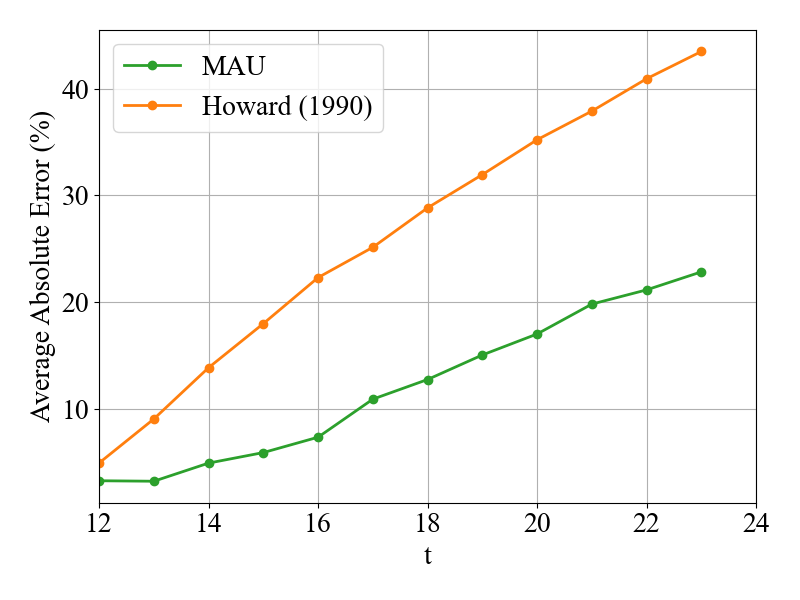
\includegraphics[width=\textwidth]{figures/exp1/lng_error_1.png}
              \caption{-90度から-54度}
              \label{fig:lng_error_1}
            \end{subfigure}
            \begin{subfigure}{0.5\textwidth}
              \centering
              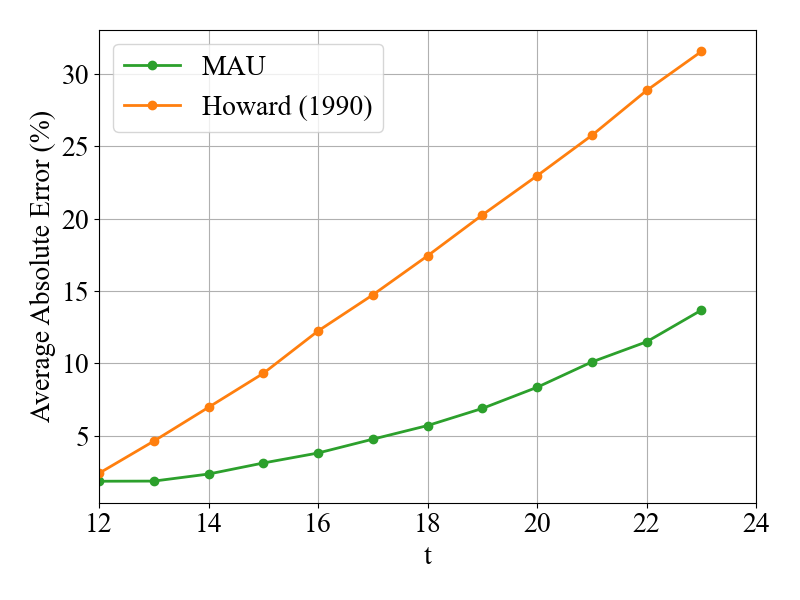
\includegraphics[width=\textwidth]{figures/exp1/lng_error_2.png}
              \caption{-54度から-18度}
            \end{subfigure} \par
            \begin{subfigure}{0.5\textwidth}
              \centering
              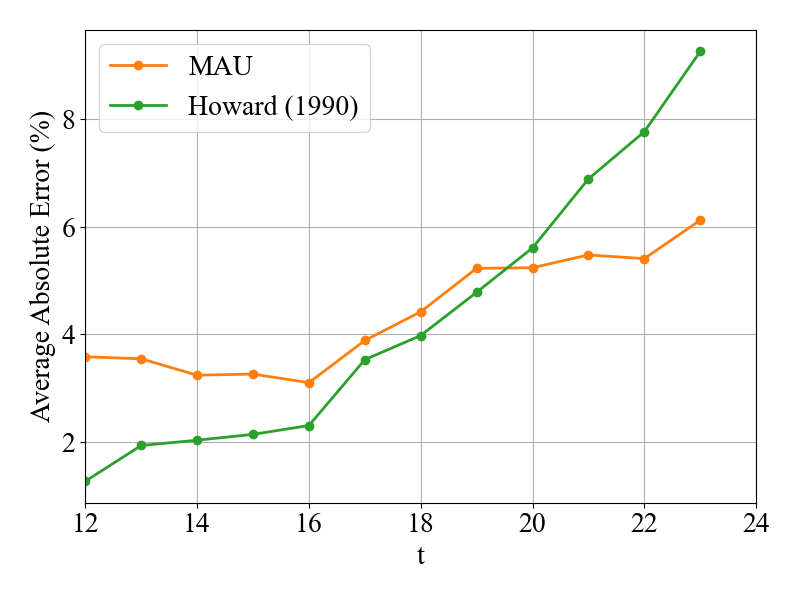
\includegraphics[width=\textwidth]{figures/exp1/lng_error_3.png}
              \caption{-18度から18度}
            \end{subfigure}
            \begin{subfigure}{0.5\textwidth}
              \centering
              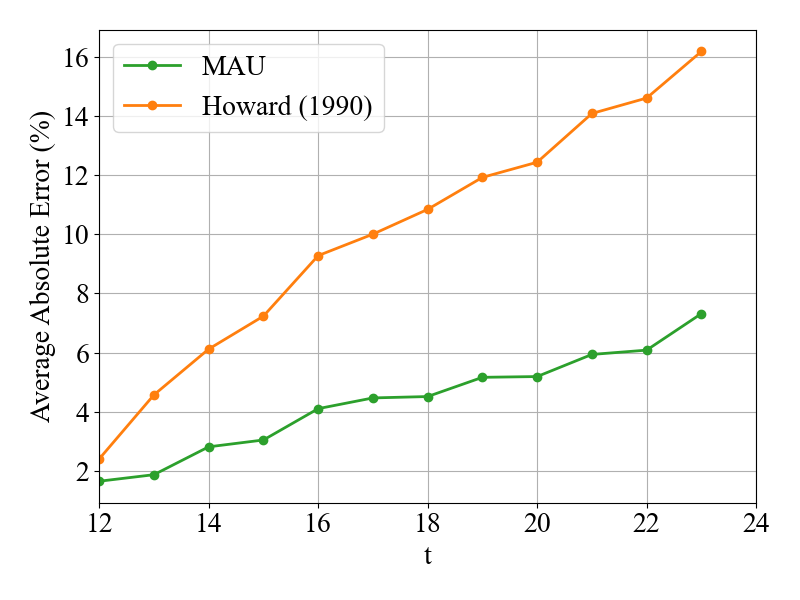
\includegraphics[width=\textwidth]{figures/exp1/lng_error_4.png}
              \caption{18度から54度}
            \end{subfigure} \par
            \begin{subfigure}{0.5\textwidth}
              \centering
              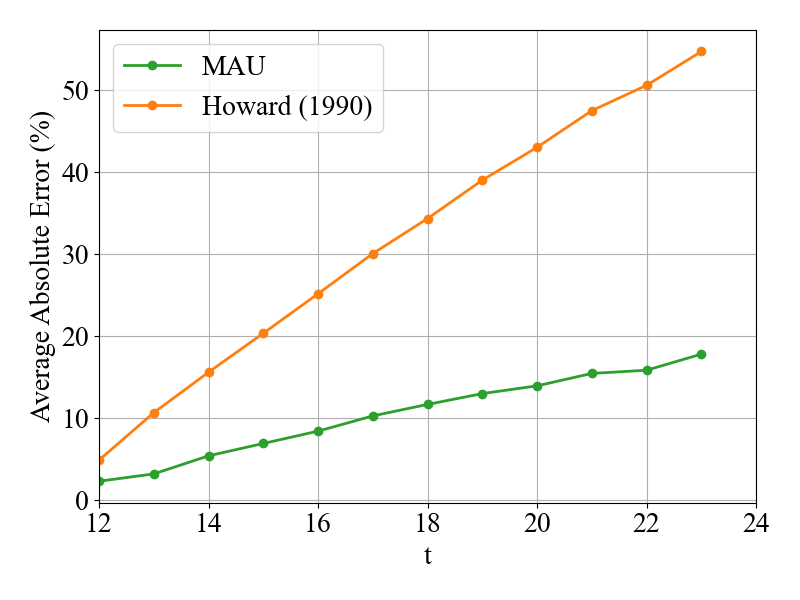
\includegraphics[width=\textwidth]{figures/exp1/lng_error_5.png}
              \caption{54度から90度}
            \end{subfigure}
            \caption{分割された各セクターにおける平均輝度の絶対誤差の時間推移。横軸が時間ステップ、縦軸が平均絶対誤差を表す。各グラフで縦軸の範囲が異なる。緑線がMAUによる予測から計算された絶対誤差、オレンジ線が単純差動回転モデルによるシミュレーションから計算された絶対誤差を表す。}
            \label{fig:lng_error}
          \end{figure}
          
        \subsubsection{画像類似度}
          全球での場合と同様に、経度ごとにも画像類似度を計算した。その時間推移を図\ref{fig:lng_ssim}に示す。同時に単純差動回転モデルの経度ごとの画像類似度も計算した。
          \begin{figure}[htbp]
            \begin{subfigure}{0.55\textwidth}
              \centering
              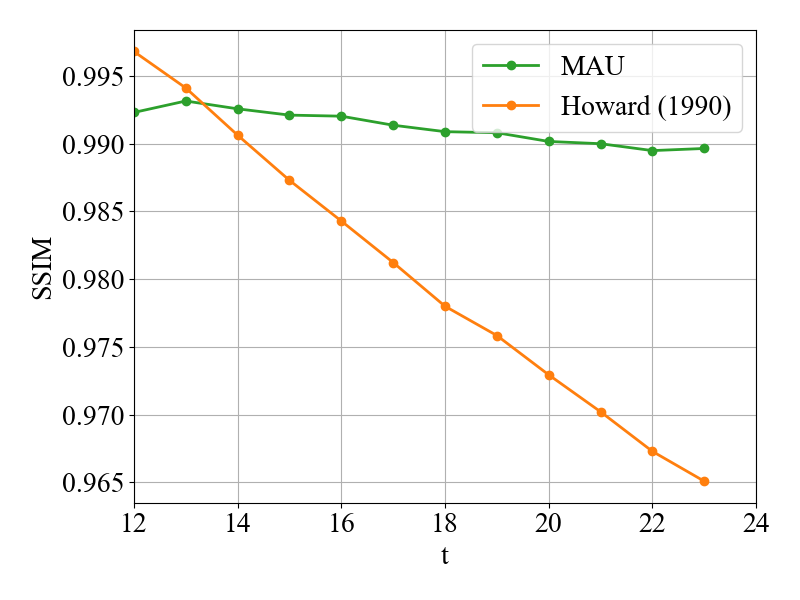
\includegraphics[width=\textwidth]{figures/exp1/lng_ssim_1.png}
              \caption{-90度から-54度}
            \end{subfigure}
            \begin{subfigure}{0.5\textwidth}
              \centering
              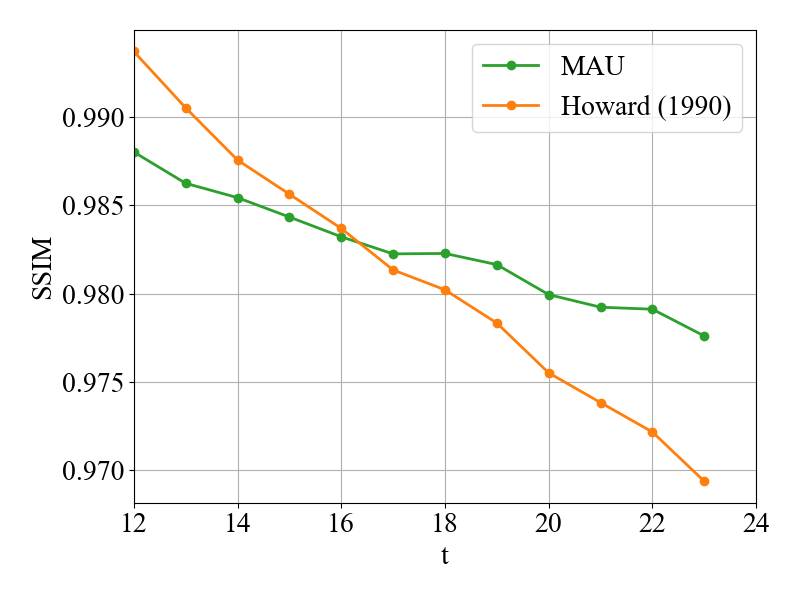
\includegraphics[width=\textwidth]{figures/exp1/lng_ssim_2.png}
              \caption{-54度から-18度}
            \end{subfigure} \par
            \begin{subfigure}{0.5\textwidth}
              \centering
              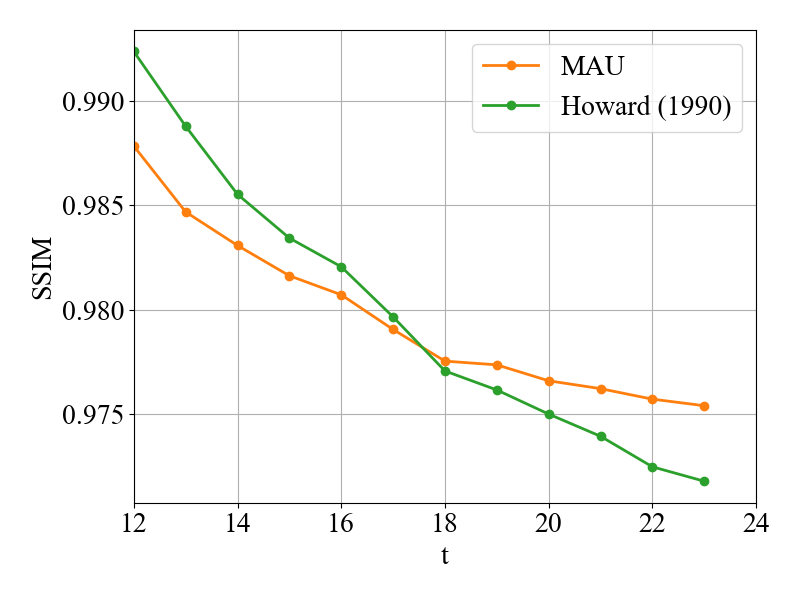
\includegraphics[width=\textwidth]{figures/exp1/lng_ssim_3.png}
              \caption{-18度から18度}
            \end{subfigure}
            \begin{subfigure}{0.5\textwidth}
              \centering
              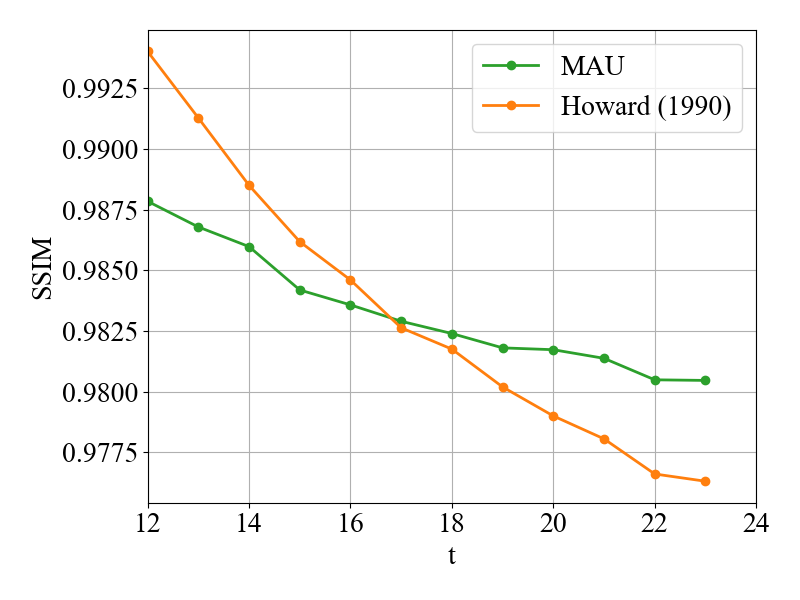
\includegraphics[width=\textwidth]{figures/exp1/lng_ssim_4.png}
              \caption{18度から54度}
            \end{subfigure} \par
            \begin{subfigure}{0.5\textwidth}
              \centering
              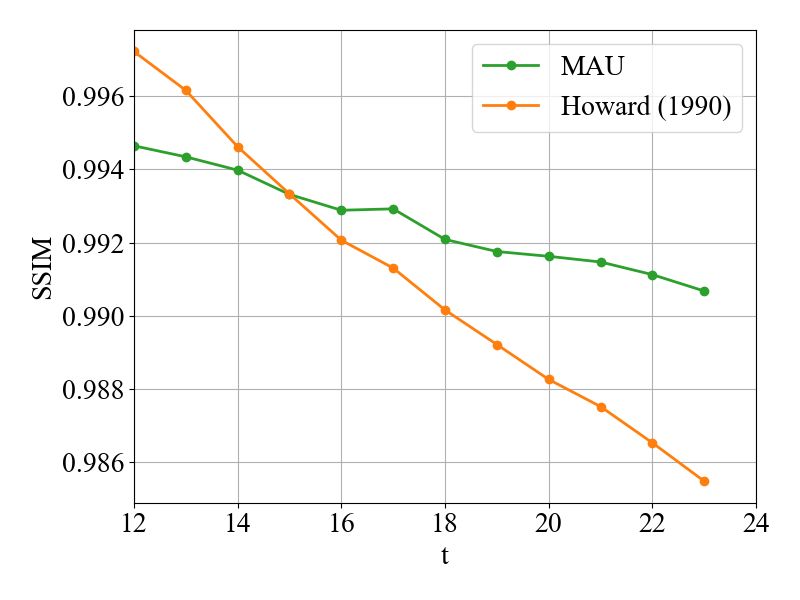
\includegraphics[width=\textwidth]{figures/exp1/lng_ssim_5.png}
              \caption{54度から90度}
            \end{subfigure}
            \label{fig:lng_ssim}
            \caption{分割された各セクターにおけるSSIMの時間推移。横軸が時間ステップ、縦軸がSSIMを表す。各グラフで縦軸の範囲が異なる。緑線がMAUによる予測から計算されたSSIM、オレンジ線が単純差動回転モデルによるシミュレーションから計算されたSSIMを表す。}
          \end{figure}

% *************************************************************************************************************
    
    \subsection{東側外縁部に対する評価}
      ここまでで、作成した動画予測モデルは、全球での平均輝度や、経度ごとの平均輝度といった定量的な評価において、実際の観測画像を正確に再現できていることを確認した。
      既存のシンプルなシミュレーションモデルとの比較でも、平均輝度の評価においては、動画予測モデルの優位性を確認できた。

      動画予測モデルのシミュレーションモデルに対するさらなる独自の特徴として、望遠鏡の視野に入っていない太陽の球面を生成することができる点が挙げられる。
      Sunpyによって提供される差動回転シミュレーションモデル\textit{physics.defferential\_rotation}は、入力された画像の全球面の各ピクセルに対して差動回転を適用することで画像を生成する。
      そのため、入力時点で望遠鏡の視野に入っていない太陽の球面を生成することができないので、より長い時間スパンでの予測を行うと、東の外縁部から徐々に予測できない領域が広がっていく。
      これに対して、動画予測モデルは、入力画像の全球面に対して特定の数理モデルを適用するのではなく、過去のデータや全体的な文脈を元に、視野に入っていなかった領域を含む未来の状態を生成する。
      
      ここでは、動画予測モデルが、そのような「入力画像の時点で全球面に見えていない領域」に対して予測能力を持つか検証を行うため、 生成された画像の東側外縁部から出現する活動領域に対する評価を行う。

      \subsubsection{視覚的評価}
        ここでは、動画予測モデルが、東側外縁部から出現する活動領域に対して、どのような予測を行っているかを視覚的に評価する。
        いくつかの例を図\ref{fig:exp1_limb_example_1}および\ref{fig:exp1_limb_example_2}に示す。ここで示す画像は、左列が入力シークエンスの最終データ、中央列がその24時間後の予測画像、右列がその48時間後の予測画像である。

        \begin{figure}[htbp]
          \centering
          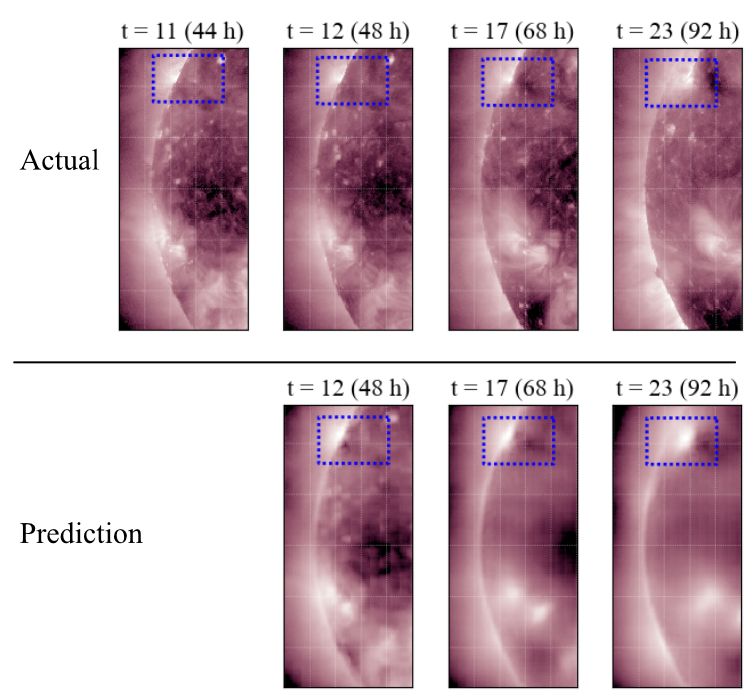
\includegraphics[width=\textwidth]{figures/exp1/limb_sample_3_caption.jpg}
          \caption{東側外縁部から出現する活動領域に対する予測の例。左列が入力シークエンスの最終データ、中央列がその24時間後の予測画像、右列がその48時間後の予測画像である。}
          \label{fig:exp1_limb_example_1}
        \end{figure}
        \begin{figure}[htbp]
          \centering
          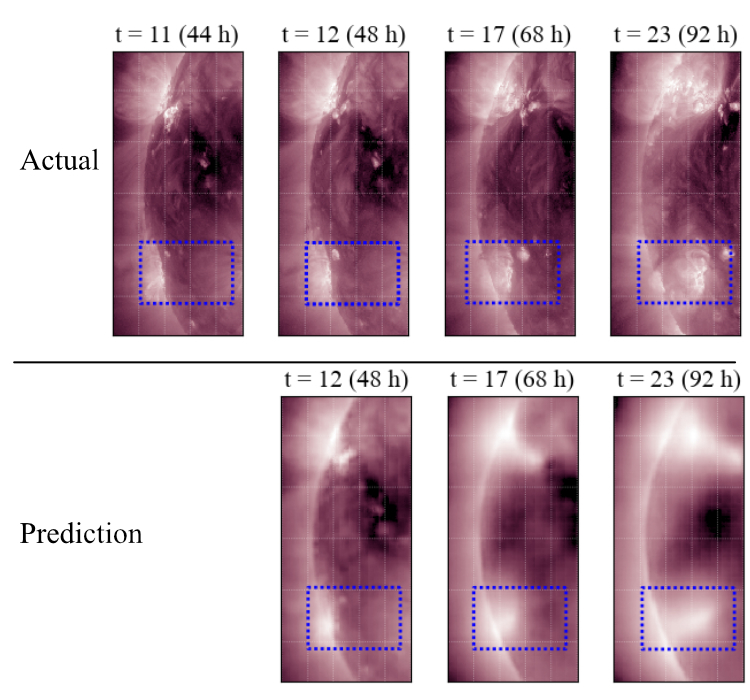
\includegraphics[width=\textwidth]{figures/exp1/limb_sample_12_caption.jpg}
          \caption{東側外縁部から出現する活動領域に対する予測の例。左列が入力シークエンスの最終データ、中央列がその24時間後の予測画像、右列がその48時間後の予測画像である。}
          \label{fig:exp1_limb_example_2}
        \end{figure}

      \subsubsection{予測対実測散布図による定量的評価}
        さらに、東側外縁部に対する評価を行うために、予測対実測の散布図を作成した。その結果を図\ref{fig:exp1_limb_scatter}に示す。
        左は、MAUによる予測画像の東側外縁部の平均輝度と、実際の観測画像の東側外縁部の平均輝度の散布図である。
        実際の観測画像の東側外縁部の平均輝度と、その48時間後の予測画像の東側外縁部の平均輝度は、相関係数0.98で、強い相関があることがわかる。
        また、最終タイムステップにおける実際の観測画像の東側外縁部の平均輝度強度が、その48時間の値とどのように一致しているかを示す散布図も作成した。その結果を右に示す。
        この散布図から、東側外縁部の平均輝度と、その48時間後の東側外縁部の平均輝度は、相関係数0.26と相関が弱く、時間経過により容易に変化することがわかる。
        これは、東側外縁部の平均輝度の変化は、単純なロジックでは予測できないことを示している。
        
        これらの結果から、動画予測モデルは、一定の複雑さを持つ東側外縁部の平均輝度に対しても、高い予測能力を持つことがわかった。
        \begin{figure}[htbp]
          \begin{subfigure}[b]{0.53\textwidth}
            \centering
            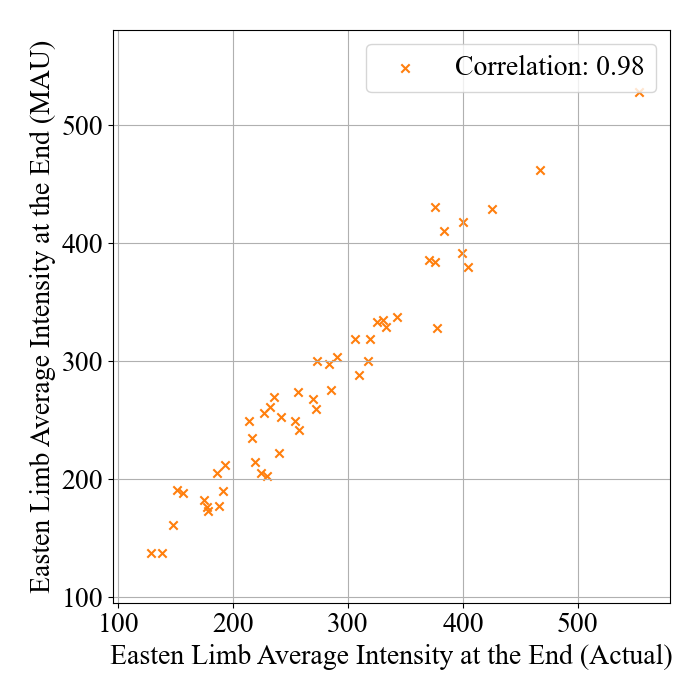
\includegraphics[width=\textwidth]{figures/exp1/limb_scatter_gt_pd.png}
            \caption{すべてのテストセットの、最終タイムステップでの東側外縁部の平均輝度の予測対実測の散布図。横軸が実際の観測画像から計算された平均輝度強度、縦軸がMAUによる予測から計算された平均輝度強度を表す。計算された相関係数は0.98である。}
          \end{subfigure}
          \begin{subfigure}[b]{0.55\textwidth}
            \centering
            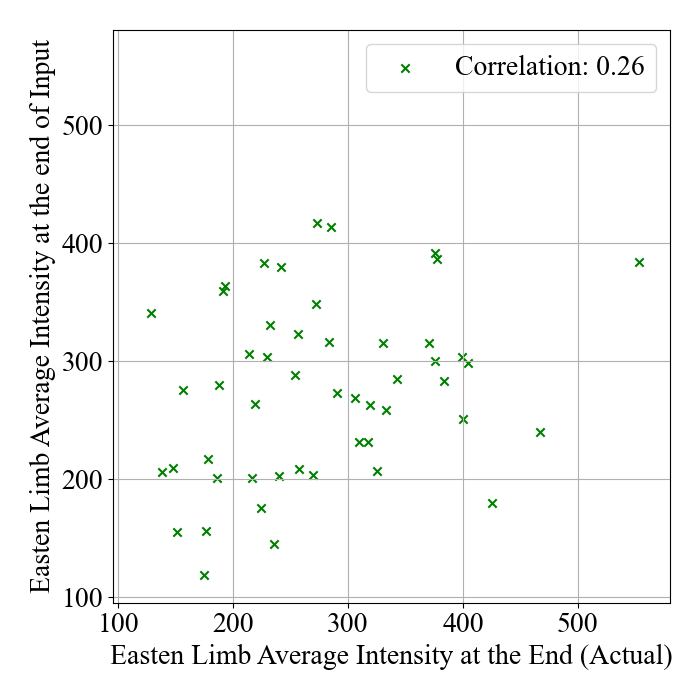
\includegraphics[width=\textwidth]{figures/exp1/limb_scatter_gt_sp.png}
            \caption{すべてのテストセットでの、最終タイムステップでの東側外縁部の平均輝度の実測値と、その48時間前の実測値の散布図。横軸が実際の観測画像から計算された平均輝度強度、縦軸がMAUによる予測から計算された平均輝度強度を表す。計算された相関係数は0.26である。}
          \end{subfigure}
          \caption{}
          \label{fig:exp1_limb_scatter}
        \end{figure}
    
    \subsection{まとめ}
      
      本実験での結果を表\ref{tab:exp1_result}にまとめる。
      \begin{table}[htbp]
        \centering
        \caption{本実験での各評価の結果。MAUは、本研究で使用した動画予測モデルによる予測に対する評価、Howard (1990)は、単純差動回転モデルによるシミュレーションに対する評価を表す。}
        \begin{tabular}{lcccccc}
        \hline
        評価指標 & 全球 & \multicolumn{5}{c}{経度ごと} \\
        \cline{3-7}
         &  & -90 to -54 & -54 to -18 & -18 to 18 & 18 to 54 & 54 to 90 \\
        \hline\hline
        平均輝度絶対誤差↓ & & & & & & \\
        \quad MAU - 1波長 & 0.05 & 0.04 & 0.03 & 0.05 & 0.06 & 0.04 \\
        \quad Howard (1990) & 0.06 & 0.05 & 0.04 & 0.06 & 0.07 & 0.05 \\
        \hline
        SSIM↑ & & & & & & \\
        \quad MAU - 1波長  & 0.9 & 0.88 & 0.89 & 0.87 & 0.85 & 0.86 \\
        \quad Howard (1990) & 0.85 & 0.87 & 0.86 & 0.84 & 0.83 & 0.85 \\
        \hline
        \end{tabular}
        \label{tab:exp1_result}
      \end{table}
       

  \section{考察}

